\begin{center}
	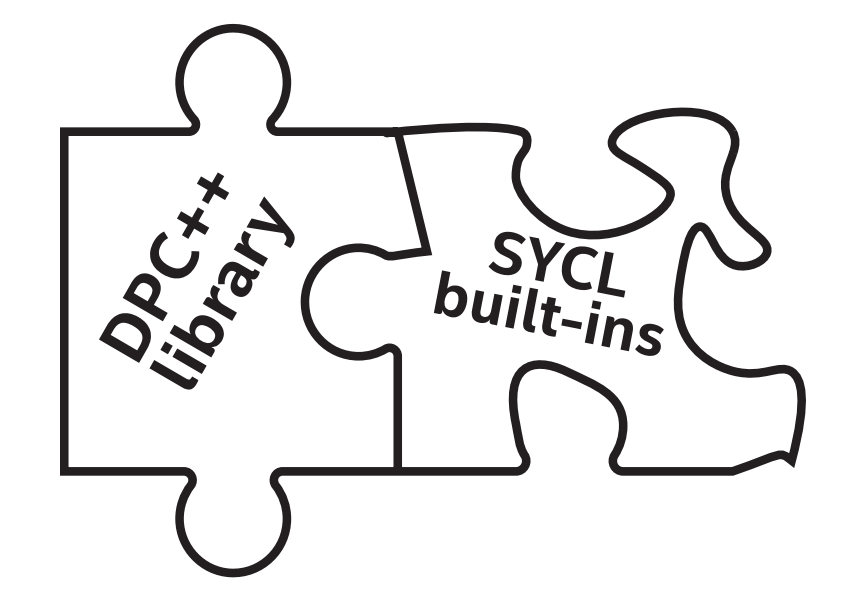
\includegraphics[width=0.5\textwidth]{content/chapter-18/images/1}
\end{center}

我们花了整本书来推广编写代码的艺术,一些优秀的程序员已经编写了我们可以直接使用的代码。库是完成工作的最好方式。这并不是懒惰的表现——这是一种比重塑他人工作更好的表现。这是一块值得拥有的拼图。\par

开源的DPC++项目包括一些库。这些库可以帮助我们使用libstdc++、libc++和MSVC库函数,甚至在内核代码中。这些库是英特尔的DPC++和oneAPI产品的一部分。这些库不绑定到DPC++编译器,因此可以与任何SYCL编译器一起使用。\par

DPC++库为创建异构应用程序和解决方案的程序员提供了另一种选择。它的API基于熟悉的标准——C++ STL、Parallel STL (PSTL)和SYCL——为开发者提供高生产率的API。这可以减少跨CPU、GPU和FPGA的编程工作,同时产生可移植的高性能并行应用程序。\par

SYCL标准定义了一组丰富的内置函数,这些函数为主机和设备代码提供了值得考虑的功能。DPC++和许多SYCL实现通过数学库实现了关键的内置函数。\par

本章讨论的库和内置函数与编译器无关。换句话说,它们同样适用于DPC++编译器或SYCL编译器。fpga\_device\_policy类用于FPGA支持的DPC++特性。\par

由于在命名和功能上存在重叠,本章将从介绍SYCL内置函数开始。\par



















